\cotefile{67}
\scanpage{86}
% archive sheet number: 88

qui opère sur $\mathrm{Oc}(V)$, opère sur $I(V)$, et on trouve

\[
\underset{\substack{\shortparallel\\\deleted{\unsure{G|V}}\operatorname{Aut}^{+}(\mathrm{Oc}(V))}}{\Gamma(V)}
\xrightarrow{\sim}\unsure{\mathfrak{S}|\mathscr{S}}_{I(V)}\,,
\]

et cet iso. \deleted{\illegible{1}} définit une structure de $V$-torseur sur $I(V)$. (Ceci résulte de la théorie combinatoire du $\unsure{N|V}$ octaèdre, ou du cube c'est kif kif.)

\uline{Proposition} \unsure{Soit|S\textsuperscript{t}} $X$ droite projective \unsure{rélles|réelle} sur un corps alg clos $k$ (il suffit qu'il \deleted{\unsure{contienne}} soit stable par extraction des racines carrées) de car. $\ne 2$, et $G=\operatorname{Aut}_{k}X$. Alors il y a corr 1-1 entre

a) les sous-groupes $V$ de $G$ isom : $\mathbb{D}_2$

b) \rule{5em}{0.4pt} $\Gamma$ de $G$ isom : $\mathfrak{S}_4$ \deleted{\unsure{non|un}}

c) les parties $S\in\mathcal{P}_6(\deleted{\unsure{S}}X(k))$ qui sont ``octaèdrales'', i.e. \deleted{telles que :} \inserted{isom :} $(\mathbb P^1_k,\{0,\infty,\pm1,\pm i\})$

par
\[
\begin{aligned}
\Gamma&=\operatorname{Nor}_{G}(V)\\
V&=\inserted{\text{unique }}\text{sous-groupe }\inserted{\text{inv. de }\Gamma,}\ \deleted{\unsure{\text{inv. de }G|\text{inv. de }\Gamma}}\ \text{isom : }\mathbb D_2\ \deleted{\unsure{\text{à }\mathbb B}}\\
S&=\text{ens de ramification de l'action de }V\text{ sur }X\\
&\hspace{2em}\deleted{\unsure{\text{ens de l'action}}},
\end{aligned}
\]

% slanted
\margin{\uline{Car} la catégorie \unsure{(au lieu précisé)|(au sens précisé)} des couples $(X,V)$ (ou $(X,\Gamma)$, $(X,S)$) $\to$ \uline{équivalente} : celle des octaèdres \uline{orientés}, une fois choisie une racine carrée de $-1$ dans $k$. Mieux : la cat des couples $(X,V)$ \unsure{est $\to$|éq $\to$} celle des couples $(\mathrm{Oc},\varphi)$ où $\mathrm{Oc}$ est un \unsure{polyèdre|octaèdre} : $\varphi:\{\pm i\}$ $\underset{=}{\sim}\,\unsure{\mathrm{or}|\omega}(\mathrm{Oc})$}

(\uline{NB} $\Gamma$ a un ens de ramification plus grand qui comprend, en plus de $S$, les ``milieux d'arêtes'' et ``centres des faces'' de l'octaèdre,

Dans une telle partie $S$, on a un antipodisme $\underline{a}_S=\underline{a}_V$ défini par la condition \deleted{\unsure{que}} pour $\sigma\in V^*$, $\underline{a}_S$ \deleted{soit} \inserted{induise} la transposition de $X^\sigma$ (de cardinal 2). On définit sur $S$ une structure octaèdrale, admettant $\Gamma$ comme groupe des autom orientés, et $\underline a$ comme antipodisme, via l'antipodisme. (les faces sont les parties $S'\in\mathcal{P}_3(S)$ telles que $S'\cup\underline a S'=S'$).

\scanpage{87}
% archive sheet number: 89

\uline{NB} On sait que la donnée d'un octaèdre \inserted{comb.} (pas orienté) revient à celle d'un système $(I,\omega)\ \deleted{\unsure{\text{dans}}}\ \mathbb{E}\mathrm{ns}_4\times\mathbb{E}\mathrm{ns}_2$, ens des codiagonales et des orientations. Ici $\omega=\{i,-i\}$, \deleted{\unsure{d'autre}} \deleted{part, la donnée de $I$ équi}\inserted{Mais ici ce n'est pas $I$} qui est donné directement, mais $S$, qui est un ens de \deleted{son} cardinal 6 sur lequel $V$ opère.

La condition à mettre \deleted{et} pour que ceci définisse une \deleted{str} structure octaèdrale (dont $S$ sera l'ens des sommets) est que $\forall\sigma\in V^*$, $\deleted{\unsure{V^\sigma|S^\sigma}}\ \operatorname{card}S^\sigma=2$, et $S=\bigcup_{\sigma\in V^*}S^\sigma$ (réunion forcément disjointe) (il s'ensuit que $\sigma$ opère sur $(S\setminus S^\sigma)$ par transposition sur \deleted{des}\inserted{chacune} deux composantes $S^{\sigma'},S^{\sigma''}$ (où $V^*=\{\sigma,\sigma',\sigma''\}$). Donc la donnée de $\deleted{\unsure{S,V\subset|S,V\hookrightarrow}}$ $(V,S,u:V\hookrightarrow\unsure{\mathfrak S|\mathscr S}_S)$, ou $(S,V\subset\mathfrak S_S)$, équivaut à celle de $S$, avec une involution sans pts fixes $a$ (ayant les $S^\sigma$ comme orbites).

Revenant à la donnée d'un $V$ qui opère \inserted{fid\textsuperscript{t}} sur $X$, considérons une orbite \inserted{$I$} de $V$ sur $X^*=X\setminus S(V)$. Donc $I$ est un torseur sous $V$. La donnée de $(X,I,I\hookrightarrow X)$ équivaut à celle de $(X,I,V(I)\hookrightarrow G_X,\text{ orbite de }V(I)\text{ dans }X)$, et on se gardera de confondre le $(V=V(I))$-torseur $I$, avec le $V$-torseur $I(V)\inserted{=I(V,X)}$ défini via l'octaèdre $\mathrm{Oc}(V)=\mathrm{Oc}(V,X)$.

En termes de $\inserted{I\deleted{\unsure{V}},\{\pm i\}}$, on peut définir un octaèdre \deleted{\uline{orienté}} comme un \deleted{\unsure{ens bine univoquement défini par la}} condition que le \deleted{groupe de ses aut.} \inserted{``l'ens de ses \unsure{4 faces|faces}'' soit ``$I$'', l'ens de ses \deleted{``pôles'' aux} orientations $\{\pm i\}$} \deleted{bi-transp} \deleted{soit $V$.} Cet \deleted{octa} octaèdre, \deleted{une fois choisie une $i=\sqrt{-1}$,} peut se réaliser canoniquement \deleted{\unsure{par des som}} comme un $(X,S)$ où $(X(I),S(I))$. On a un isom can

\scanpage{88}
% archive sheet number: 90

\[
X(I)/V(I)\simeq X(J)\qquad\text{où }J=J(I)\text{ comme dessus}
\]

Ceci dit soit \deleted{$I\hookrightarrow X$ on \unsure{a donc|se donne} donc dans $X$ une opération $V=V(I)$}\inserted{une opération de $V$ sur $X$} $V\hookrightarrow G_X$, d'où un $I(V)$ $V$-torseur des bi-faces de $\mathrm{Oc}(V)$, et on a \deleted{$X\simeq$}

\[
X\simeq X(I(V))\qquad\text{iso. canonique}
\]

(et non $X\simeq X(I)$). Mais pour \deleted{un} deux torseurs $T,T'$ sous un $=$ $V$, on aura

\[
X(T\wedge T')=X(T)\wedge_V T'
\]

\margin{à expliciter}

Soit donc
\[
\begin{aligned}
\underline{t}=\delta(I,\unsure{X|\lambda})&\text{ le }V\text{-torseur tel que }I(V)\simeq I\wedge_V\tau\\
&\text{i.e. }\tau\simeq I(V)\wedge I^{-1}
\end{aligned}
\]

on aura donc

\[
\boxed{X=X(I(V))=X(I)\wedge_V\underline t}
\]

\deleted{Donc} \deleted{et l'on a} \inserted{donc}

\[
\boxed{X/V\simeq X(I)/V\simeq \deleted{X}Z(J)}
\]

En résumé :

\uline{\unsure{bis|Loi|Cor.} : Prop} \deleted{La donnée, d'une part $V=\mathbb D_2$} \inserted{Pour $I\in\operatorname{Ob}\mathbb E\mathrm{ns}_4$} donné, d'où $J$ et $V=V(I)$, la donnée de un $X$ et d'un plongement $V\subset \deleted{\unsure{V_X|G}}G_X$ équivaut à la donnée d'un torseur $\underline t$ sous $V$,

\[
\text{via}\qquad \tau\longmapsto X(I)\wedge_V\deleted{\tau}\underline t
\]

\[
\text{On a alors}\qquad X/V\simeq\deleted{X}Z(J)\qquad\text{(iso. canonique).}
\]

\deleted{\uline{Corollaire}} \inserted{Donc} la donnée de $(X,I\hookrightarrow X)$ équivaut à celle de a) un pts $\zeta$ \unsure{de|/ de} $Z(J)^*$, b) un $V$-torseur $\underline t$, \deleted{c) Un $V$-isom \unsure{un|tel} tel que $X=X(I)\wedge_V\underline t$, et} \deleted{un \unsure{espace}.} \deleted{$X_\zeta=$ fibre} de \unsure{.} $X_\zeta=X(I)_\zeta\wedge\underline t\simeq I$ i.e. $\underline t=I\wedge X(I)_\zeta^{-1}$

\scanpage{89}
% archive sheet number: 91

\uline{Théorème} \unsure{Soit|Soient} $k$ un corps alg. clos de car. $\ne 2$, \deleted{Soit $I$ un ens de card 4, d'où $J$ de card. 3, et $V=V(J)$.} \deleted{Considérons}

Considérons le groupoïde des $(X,I\hookrightarrow X)$, où $X$ est une droite projective sur $k$, \deleted{telle} \inserted{$I$ de card 4.} Ce groupoïde est équivalent à celui des couples $(I,\zeta\in Z(J(I))^*)$, en associant à ce couple

\[
X=X(I)\wedge_{\underset{\text{ou }V(I)}{\underbrace{V(J(I))}}}t(\zeta,I)
\qquad\begin{aligned}&\text{où }t(\zeta,I)\text{ est le }V(I)\text{-}\\[-2pt]&\text{torseur }\ I\wedge X(I)_\zeta^{-1}\end{aligned}
\]

$\deleted{\unsure{Z}}I\hookrightarrow X$ est la fibre \inserted{$X_\zeta$} de $X$ en $\zeta$, compte tenu que

\[
\begin{aligned}
X/V(I)&\simeq X(I)/V(I)\simeq\deleted{X}Z(J)\\
X_\zeta&\simeq X(I)_\zeta\wedge t(\zeta,I).
\end{aligned}
\]

\deleted{\unsure{Cor|Si|NB}} Si $I$ est muni d'un pt $i_0$, on a une description de $X$ comme $X(I)\wedge_{V(I)}X(I)_\zeta^{-1}$, c'est isom. à $X(I)$ une fois choisi un sommet de $X(I)$ au dessus de $\zeta$.

De façon plus générale, \deleted{\unsure{pour|pour un|en}} la donnée d'un isom. ``admissible'' $X\simeq X(I)$ équivaut à celle d'un $V$-isom $I\simeq\deleted{\unsure{I|Z}}X(I)_\zeta$.

\scanpage{91}
% archive sheet number: 93

% slanted
\margin{\uline{Déc 83}}

\uline{Courbes elliptiques réelles}

Soit $k$ un anneau (\unsure{présumé|disons|par exemple} comm.) \deleted{$M$ un $k$-\unsure{mo}} Considérons la catégorie des $k$-Modules $M$ munis d'un autom $\sigma$ \deleted{tel q} tels que

a) $\sigma^2=\mathrm{id}$

b) $2\mathrm{id}_M$ injectif (on dit alors $M$ 2-régulier)

A un tel couple $(M,\sigma)$, \inserted{nous} associons \deleted{\unsure{les}} couples $(P,Q,m)$ de deux \inserted{$k$-}modules pour lesquels $2\mathrm{id}_P$ et $2\mathrm{id}_Q$ sont injectifs (i.e. $P,Q$ 2-réguliers), et $m\subset P/2P\oplus Q/2Q$ \inserted{sous $k/2k$-module} avec $m\cap P/2P=0$, $m\cap Q/2Q=0$ (soit deux sous-modules $p'\subset p\overset{\mathrm{déf}}=P/2P$, $q'\subset q=Q/2Q$, et un iso. $p'\simeq q'$), de la façon suivante

\[
\begin{aligned}
P&=M_+=\operatorname{Ker}(\mathrm{id}_M-\sigma)=\{x\in M\mid\sigma x=x\}\\
Q&=M_-=\operatorname{Ker}(\mathrm{id}_M-\sigma)=\{\unsure{n|x}\in M\mid\sigma x=-x\}
\end{aligned}
\]

\unsure{NB|N.B.} $M_+\cap M_-=0$ dans $M$, car $M$ 2-régulier, et on \margin{!} a $2M\subset M_+\oplus M_-\hookrightarrow M\deleted{\subset\tfrac12(M_+\oplus M_-)}$ car $\forall x\in M$, on a $2x=(\underset{M_+}{\underbrace{x+\sigma x}})+(\underset{M_-}{\underbrace{x-\sigma x}})$

soit
\[
\underset{\substack{\shortparallel\\2M}}{M'}\subset M_+\oplus M_{\unsure{1|-}}=P\oplus Q\qquad d'
\]

on a donc
\[
\deleted{\unsure{M'\hookrightarrow}}2P\oplus 2Q\subset M'\subset P\oplus Q
\]

donc $M'$ est l'image d'un sous-module $m$ de $(P\oplus Q)/2P\oplus 2Q\simeq\underset p{\underbrace{P/2P}}\oplus\underset q{\underbrace{Q/2Q}}$, et on vérifie \deleted{\unsure{que}}

\[
\begin{aligned}
\left\{\begin{aligned}m\cap\deleted{\unsure{q}}p&=0\\m\cap q&=0\end{aligned}\right.
&\quad\begin{aligned}
\text{i.e. } \underset{M'\cap P+(2P+2Q)}{\underbrace{M'\cap(P+(2P+2Q))}}&=(2P+2Q)\\
\text{i.e. }M'\cap(Q+(2P+2Q))&=2Q
\end{aligned}
\end{aligned}
\]
car $M'\cap P=2P$ puisque $2x\in P$ i.e. $2\sigma x=2x$ implique $x\in P$ i.e. $\sigma x=x$, et $M'\cap Q=2Q$.

D'ailleurs \deleted{\unsure{$M'\subset P\oplus Q$}} $(M,\sigma)$ se reconstitue à isom can près via $(P,Q,m)$, car $M'\subset P\oplus Q$ se reconstitue, et \deleted{\unsure{$M'$}}$\sigma_{M'}$ aussi bien entendu par $\mathrm{id}_P\oplus(-\mathrm{id}_Q)$), or $2\mathrm{id}_M\deleted{\unsure{4p}}:M\to M'$ est un iso de $(M,\sigma_M)$ avec $(M',\sigma_{M'})$.

\uline{Prop} Le foncteur précédent $(M,\sigma)\longmapsto(P,Q,m)$ est une équivalence

\uline{Cor} Supposons $k$ \deleted{\unsure{qui|soit}} \inserted{comm.} \deleted{intègre et \unsure{régulier} et ppal}\inserted{$I$ de Dedekind, avec \deleted{$k$}$k$ 2-régulier}, prenons \deleted{des} $M$ \deleted{libres} \inserted{projectifs} de \deleted{rang}\inserted{rg} 2 avec $\sigma\ne\mathrm{id}_M,-\mathrm{id}_M$, alors la cat \deleted{de ces}\inserted{des} foncteurs \deleted{équivaut à celle}\inserted{$(M,\sigma)$ avec, où $M$ fid\textsuperscript{t} de rg 2,} équivaut à celle des paires $(P,Q)$ avec $P,Q$ inv., et $p'\subset P/2P$, $q'\subset Q/2Q$ et $p'\overset u\simeq q'$ donné.

\scanpage{92}
% archive sheet number: 94

% printed form
{\scriptsize
\begin{verbatim}
//*   CRAY2   0344        I
           00000000      00000000    555555555555       11
         0000000000    0000000000   555555555555      111
       00      0000  00      0000  55               1111
      00     00 00  00     00 00  55                 11
     00    00  00  00    00  00  55                 11
    00   00   00  00   00   00  555555555          11
   00  00    00  00  00    00  5555555555         11
  00 00     00  00 00     00           55        11
 0000      00  0000      00            55       11
000       00  000       00            55       11
0000000000    0000000000   555555555555   1111111111
00000000      00000000    55555555555    1111111111
\end{verbatim}
}

\handwritten{\[
\deleted{M'}\quad P\oplus Q\supset M'\supset 2P\oplus 2Q
\]}

\handwritten{\[
\begin{aligned}\sigma(x,y)&=x-y\\(1+\sigma)(x,y)&=2x\\(1\deleted{\unsure{+}}-\sigma)(x,y)&=2y\end{aligned}
\]}

\handwritten{\[
\begin{aligned}
&\deleted{\unsure{1+2|1+}}\\
&\deleted{\unsure{\forall x\in P,\ \exists\,2y\in M'\!Q|\forall x\in P,\ \exists\,y\in M'|\exists\,x,y\in M'},\ (1+\sigma)(x,y)=x\quad\text{i.e. }2x}\\
&P=\quad\deleted{x\in\ (x,y)\in M'}\\
&\deleted{(x,y)}\,x+2y\in M'
\end{aligned}
\]}

\handwritten{\[
\left\{\begin{aligned}M'\cap P&=2P\\M'\cap Q&=2Q\end{aligned}\right.
\qquad\text{i.e. }\underset{=(M'\cap P)+2Q}{\underbrace{M'\cap(P+2Q)}}=2P+2Q
\]}

{\scriptsize
\begin{verbatim}
 CCCCCCCCCC   RRRRRRRRRRR    AAAAAAAAAA   YY        YY   2222222222
CCCCCCCCCCCC  RRRRRRRRRRRR  AAAAAAAAAAAA  YY        YY  222222222222
CC        CC  RR        RR  AA        AA   YY      YY             22
CC            RR        RR  AA        AA    YY    YY              22
CC            RR        RR  AA        AA     YY  YY               22
CC            RRRRRRRRRRRR  AAAAAAAAAAAA      YYYY               22
CC            RRRRRRRRRRR   AAAAAAAAAAAA       YY              22
CC            RR    RR      AA        AA       YY            22
CC            RR     RR     AA        AA       YY          22
CC        CC  RR      RR    AA        AA       YY        22
CCCCCCCCCCCC  RR       RR   AA        AA       YY       222222222222
 CCCCCCCCCC   RR        RR  AA        AA       YY       222222222222
\end{verbatim}
}

\handwritten{\[
\begin{aligned}
&m\subset\underset p{\underbrace{P/2P}}\times\underset q{\underbrace{Q/2Q}}\\
&\hspace{4em}\text{sous-module}\\
&\hspace{6em}\text{de }k/2k\text{-module}\\
&m\cap p=0\qquad m\to p\ \text{injectif}\\
&m\cap q=0\qquad m\to q\ \text{injectif}
\end{aligned}
\]}

{\tiny
\begin{verbatim}
****A  START  JOB  344  CRAY2       ROOM     3.08.27 PM 19 AUG 82  R6.PR1    SYS JES2  JOB  344  START  A****
****A  START  JOB  344  CRAY2       ROOM     3.08.27 PM 19 AUG 82  R6.PR1    SYS JES2  JOB  344  START  A****
****A  START  JOB  344  CRAY2       ROOM     3.08.27 PM 19 AUG 82  R6.PR1    SYS JES2  JOB  344  START  A****
****A  START  JOB  344  CRAY2       ROOM     3.08.27 PM 19 AUG 82  R6.PR1    SYS JES2  JOB  344  START  A****
****A  START  JOB  344  CRAY2       ROOM     3.08.27 PM 19 AUG 82  R6.PR1    SYS JES2  JOB  344  START  A****
****A  START  JOB  344  CRAY2       ROOM     3.08.27 PM 19 AUG 82  R6.PR1    SYS JES2  JOB  344  START  A****
\end{verbatim}
}

{\scriptsize
\begin{verbatim}
DERNIERE MISE A JOUR DE JOURNAL : 11-08-82
ATTENTION .........
   ]         UN ARRET EXCEPTIONNEL POUR PREPARER L'ARRIVEE DE NOUVELLES
   ]         UNITES AURA LIEU DU VENDREDI 20 AOUT A 17H 30 AU LUNDI
   ]         23 AOUT A 8H.
\end{verbatim}
}

\handwritten{$x\mapsto 2x:M\to M$ injectif. \deleted{$k[\frac12$} \uline{$M$ plat sur $k$} donc $x\mapsto 2x$ $M\to M$ injectif}

\handwritten{\deleted{\[
\begin{aligned}
&\deleted{\unsure{k'=k\hookrightarrow}}\ k'=k[\tfrac12]\\
&M\subset M\otimes k'=M'=M'_+\oplus M'_-=\deleted{M_+ k'}\\
&M_+=\{m\in M\mid\sigma x=\unsure{x|+}\}=\operatorname{Ker}(1-\sigma)\\
&M_-=\{m\in M\mid\sigma x=-x\}=\operatorname{Ker}(1+\sigma)
\end{aligned}
\]}}

\handwritten{\[
\begin{aligned}M_+\cap M_-&=0\\
M/M_++M_-&\quad\text{annulé par }2\\
2x&=(\underbrace{x+\sigma x}_{\in M_+})+(\underbrace{m-\sigma x}_{\in M_-})
\end{aligned}
\]}

\handwritten{\deleted{\[
\begin{aligned}
&M_+\oplus M_-\subset M\subset\tfrac12(M_+\oplus M_-)\quad\deleted{\unsure{ou}}\\
&2M_++2M_-\subset\deleted{\unsure{2}}\underset{M'}{\underbrace{2M}}\subset M_+\oplus M_-
\end{aligned}
\]}}

\handwritten{\[
\begin{aligned}
&\deleted{P\ Q}\quad P,Q\qquad M\\
&m\in P/2P\oplus Q/2Q\\
&(1+\sigma)M'=2M_+\qquad(1\deleted{\unsure{+}}-\sigma)M'=2M_-
\end{aligned}
\]}

\scanpage{93}
% archive sheet number: 95

\uline{Courbes elliptiques réelles} \deleted{Elles sont} La catégorie \unsure{de|des} ces courbes (avec morphismes pas néc. des iso) revient à celle des \deleted{\unsure{$\pi$|$p$}} systèmes $(\pi,\sigma,c)$, où $\pi$ est un $\mathbb Z$-module libre, \inserted{de rg $2$} \deleted{$\sigma$ une} $c$ une structure \deleted{conf} conforme orientée sur $\pi_{\mathbb R}=\pi\otimes_{\mathbb Z}\mathbb R$, et $\sigma$ un anti-automorphisme du syst. $(\pi,c)$, qui peut s'interpréter comme une involution de $\pi$, renversant l'\uline{orientation} \inserted{de $\pi\otimes_{\mathbb Z}\mathbb R$ i.e. de déterminant $-1$} (donc $\ne\pm\mathrm{id}_\pi$), et conservant la structure conforme.

Pour le couple $(\pi,\sigma)$ il y a exactement deux possibilités, à iso. près. \deleted{Pour} (elles sont d'ailleurs isogènes...). Il reste, pour chacune d'elles, à trouver les structures conformes qui sont invariantes par $\sigma$. On peut les normaliser par \deleted{$\unsure{\sigma Q=Q|\sigma Q=\sigma}$}

\[
Q(u_+)\deleted{(=Q(v))}=1
\]

\margin{\uline{NB}\quad $u_+$ est une base de $\pi_+$\\ $u_-$ \rule{6em}{0.4pt} $\pi_-$}

donc ce sont les structures de la forme

\[
Q(xu_++yu_-)=x^2+ay^2
\]

où $a\in\mathbb R^{*+}$. Il y a donc deux familles de courbes elliptiques réelles, paramétrées chacune par $\mathbb R^{*+}$, on peut les désigner par $E_a,E'_a$ ($a\in\mathbb R^{*+}$). \deleted{Considérons}

Considérons les autom \deleted{de ces cour} \inserted{d'une courbe elliptique} définie par $(\pi,\sigma,c)$, ils correspondent aux \deleted{\unsure{un tel doit|un tel est}} autom $\theta$ de $\pi$ qui a) commutent à $\sigma$ et b) respectent la structure conforme \inserted{orientée} $c$, \deleted{\unsure{en particulier|ce qui peut s'interpréter|ou plutôt}} ou ce qui revient au $=$ (étant d'ordre fini) la forme $Q$ \inserted{(en plus de l'orientation)}. \deleted{Donc} $\theta$ transforme $\pi^{+}_{-}$ en $\pi^{+}$, \deleted{Montrons la symétrie centrale} \deleted{\unsure{fixe|ainsi que}} \inserted{il transforme la $\unsure{2^{\text{de}}|1^{\text{ère}}}$} en un multiple \inserted{soit} $\pm e_0$, $\unsure{\mathrm{OPS}|\mathrm{DPS}}$ quitte à composer avec la symétrie \unsure{centrale $-1$)|(\mbox{i.e.} de $-1$)} que c'est $e_0$. Mais les seul autom de $\mathbb R e_0+\mathbb R e_1$ qui respecte $Q$, qui fixe $e_0$ et qui n'est pas l'identité, est $\sigma$, \deleted{\unsure{qui inverse|précisément}} \inserted{or il} inverse l'orientation ! Donc il n'y a que l'autom universel, correspondant à $-\mathrm{id}_{\unsure{\pi|V}}$.

\scanpage{94}
% archive sheet number: 96

Pour une courbe elliptique \uline{conforme} donnée, définie par un réseau \inserted{$\pi$} dans un espace vectoriel complexe \inserted{$V$} de dim $1$, les structures réelles qu'on peut mettre dessus correspondent aux \deleted{\unsure{orientations|involutions}} \inserted{droites réelles} de $V$, telles que la \deleted{symétrie} \inserted{réflexion} orth. par r. à $\mathbb D$ conserve $\pi$. Peut-il y en avoir plusieurs ? Si oui, les structures réelles correspondantes sont elles isom (i.e. conjuguées de l'une d'elles par les autom complexes de la courbe) ?

\deleted{En tous cas, si $\sigma,\sigma'$ sont les autom \unsure{involutifs des|involutifs de}} \deleted{Cas de}

Dans tous les cas, soit $G$ le groupe des autom \uline{conformes} de la courbe elliptique conforme \inserted{$X$ définie par} $(\pi,c)$. Pour que \deleted{l'on Pour que} $X$ admette une structure réelle, il \uline{faut} en tous cas que $G\xrightarrow{\det}\pm1$ soit surjectif, de sorte qu'on a un

\diagram{\begin{tikzcd}[ampersand replacement=\&,column sep=small,row sep=tiny]
1 \arrow[r,dash] \& G^+ \arrow[r] \arrow[d,equal] \& G \arrow[r] \& \pm1 \arrow[r,dash] \& 1\\
\& \mathrm{Aut}(X) \& \& \&
\end{tikzcd}}

Mais un élément $\sigma$ de $G$ de déterminant $-1$ est une transformation orth. de déterminant $-1$, c'est néc. une réflexion, donc c'est une structure réelle sur la courbe elliptique : les courbes elliptiques qui admettent une structure réelle sont donc celles isom à la conjuguée, i.e. celles dont l'invariant modulaire est \uuline{réel}. L'ens \deleted{de ces structures} \deleted{\unsure{s'identifie à $G^-$ est|s'identifie à $G^-$}} \deleted{(sur $X$ fixée) est un torseur sous $G^+$, qui} \inserted{$G^+$ est cyclique d'ordre} \deleted{pour $g$ \unsure{fixé|fini}, a} $n=2,4$ ou $6$, et $G$ \deleted{est isom} avec sa structure d'extension est isomorphe au groupe diédral $D_n$. L'ens des

\scanpage{95}
% archive sheet number: 97

structures réelles s'identifie à $G^-$, qui est un \uline{torseur} sous $G^+$ par translation à gauche. Par contre, l'opération de $G^+$ sur $G^-$ par autom intérieurs n'est pas libre, le centre $Z=\{\pm1\}$ de $G$ opère trivialement, et il y a deux orbites sous $G^+$ (ou mieux $G^+/Z$)

\deleted{Donc on trouve} les $2$ \unsure{st|et} \inserted{(pour $n=4$ ou $6$)} les symétries par rapp. respectivement aux sommets et aux arêtes des \deleted{\unsure{ca|co}} polygones (carré ou hexagone) \unsure{fondamentaux|fondamental}.

\figure{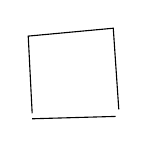
\begin{tikzpicture}[x=1cm,y=1cm]\draw (0,0.05) -- (-0.05,1.03) -- (1.03,1.13) -- (1.10,0.10);\draw (0,-0.02) -- (1.06,0.01);\end{tikzpicture}}

\uline{Donc} on résume

\uline{Proposition}. Soit une courbe elliptique \deleted{réelle} complexe. \deleted{Pour qu'elle admette une} Les structures réelles \inserted{sur $X$} \deleted{\unsure{qu'il s|i.e.}} \deleted{qu'elle} correspondent aux \inserted{anti} autom \deleted{\unsure{involutifs|involutif}} de la courbe \inserted{elliptique} conforme \deleted{positive ?} \deleted{qu'il y en a} et il y en a si et seulement si la suite

\diagram{\begin{tikzcd}[ampersand replacement=\&,column sep=small]
1\arrow[r,dash]\&G^+\arrow[r,dash]\&G\arrow[r,dash]\&\pm1,\arrow[r,dash]\&\unsure{1|\phi}
\end{tikzcd}}

est exacte (à droite). Dans ce cas, $G$ est \inserted{isom au} \deleted{au} groupe diédral \inserted{$D_n$} dont $G^+$ (d'ordre \inserted{$n=$}$2,4$ ou $6$) est le groupe des rotations. L'ens des structures réelles se partage en deux orbites sous $G^+$, (opérant par autom intérieurs), et les structures réelles correspondant à deux orbites distinctes sont (par définition !) non isomorphes. \deleted{et les deux orbites correspondent aux structures $E_a,E'_a$}

Je présume que si l'une est formé de structures $E_a$ ($a\in\mathbb R^{*+}$ fixé), l'autre est formé des structures $E'_a$ (avec le $=$ $a$), et inversement, i.e. qu'on peut trouver un $a\in\mathbb R^{*+}$ unique, tel que les deux orbites sont l'une formée des structures isom à $E_a$, l'autre des structures isom à $E'_a$. De plus il faudrait.

\scanpage{96}
% archive sheet number: 98

% printed form
{\scriptsize
\begin{verbatim}
//*   FATAR   0338        I
           00000000      00000000      00000000     2222222222
         0000000000    0000000000    0000000000   222222222222
       00      0000  00      0000  00      0000  22        22
      00     00 00  00     00 00  00     00 00           22
     00    00  00  00    00  00  00    00  00           22
    00   00   00  00   00   00  00   00   00          22
   00  00    00  00  00    00  00  00    00        22
  00 00     00  00 00     00  00 00     00      22
 0000      00  0000      00  0000      00    22
000       00  000       00  000       00   22
0000000000    0000000000    0000000000   222222222222
00000000      00000000      00000000    222222222222
\end{verbatim}
}

{\scriptsize
\begin{verbatim}
FFFFFFFFFFFF   AAAAAAAAAA   TTTTTTTTTTTT   AAAAAAAAAA   RRRRRRRRRRR
FFFFFFFFFFFF  AAAAAAAAAAAA  TTTTTTTTTTTT  AAAAAAAAAAAA  RRRRRRRRRRRR
FF            AA        AA       TT       AA        AA  RR        RR
FF            AA        AA       TT       AA        AA  RR        RR
FF            AA        AA       TT       AA        AA  RR        RR
FFFFFFFF      AAAAAAAAAAAA       TT       AAAAAAAAAAAA  RRRRRRRRRRRR
FFFFFFFF      AAAAAAAAAAAA       TT       AAAAAAAAAAAA  RRRRRRRRRRR
FF            AA        AA       TT       AA        AA  RR    RR
FF            AA        AA       TT       AA        AA  RR     RR
FF            AA        AA       TT       AA        AA  RR      RR
FF            AA        AA       TT       AA        AA  RR       RR
FF            AA        AA       TT       AA        AA  RR        RR
\end{verbatim}
}

% crop-candidate: scan 96
\figure{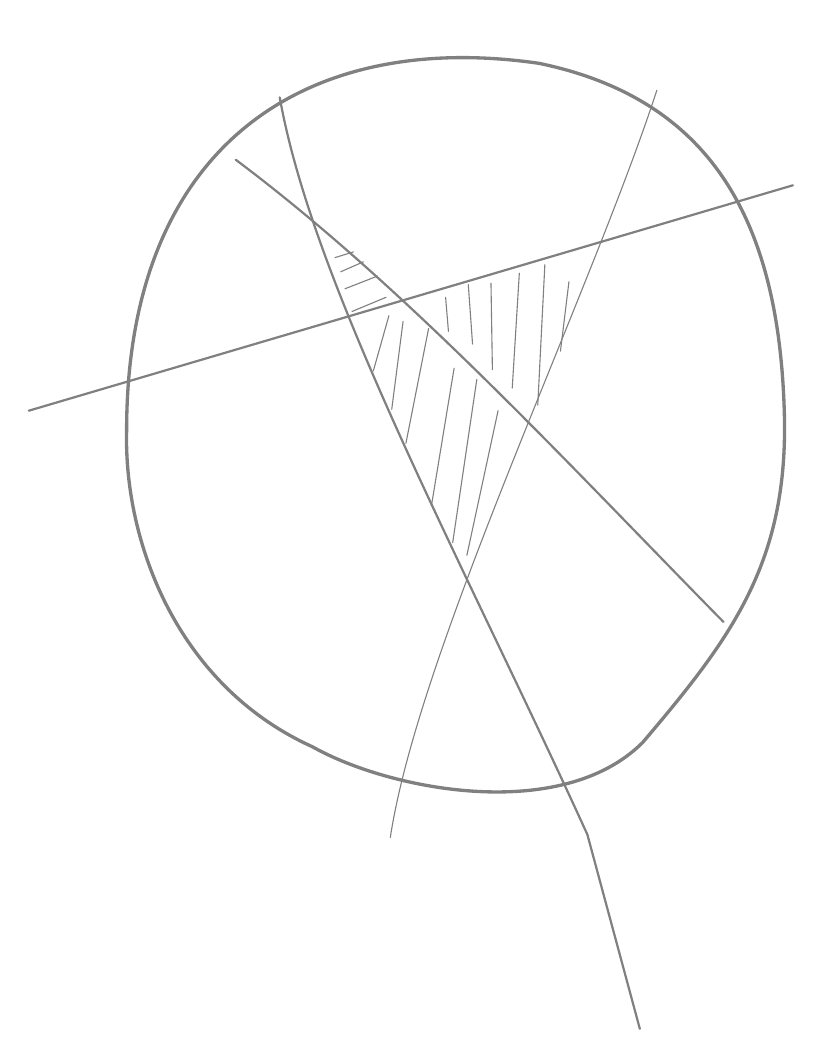
\begin{tikzpicture}[x=0.018cm,y=-0.018cm,line cap=round,line join=round]
\draw[gray,line width=1.2pt] (784,320) .. controls (784,119) and (910,37) .. (1075,61) .. controls (1200,87) and (1245,177) .. (1248,311) .. controls (1250,414) and (1210,467) .. (1148,540) .. controls (1091,597) and (970,574) .. (915,543) .. controls (820,500) and (782,399) .. (784,320) -- cycle;
\draw[gray,thick] (861,129) .. controls (981,219) and (1092,340) .. (1205,455);
\draw[gray,thick] (892,85) .. controls (916,220) and (1024,418) .. (1109,605) -- (1146,742);
\draw[gray] (1158,80) .. controls (1111,224) and (990,475) .. (970,607);
\draw[gray,thick] (715,306) -- (1254,147);
\draw[gray] (931,198)--(944,194) (935,208)--(951,201) (938,220)--(961,211) (943,236)--(967,226) (969,239)--(958,278) (979,243)--(971,305) (997,248)--(981,329) (1015,276)--(999,373) (1031,284)--(1014,399) (1046,306)--(1024,408) (1009,226)--(1011,250) (1025,217)--(1028,259) (1041,216)--(1042,277) (1061,209)--(1056,290) (1079,203)--(1074,302) (1096,215)--(1090,264);
\end{tikzpicture}}

% crop-candidate: scan 96
\figure{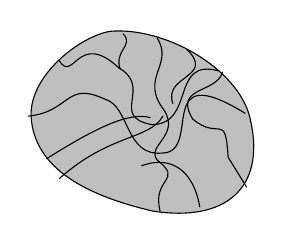
\begin{tikzpicture}[x=0.018cm,y=-0.018cm,line cap=round,line join=round]
\draw[fill=gray!50] (123,374) .. controls (122,343) and (162,315) .. (181,314) .. controls (221,312) and (272,343) .. (278,378) .. controls (288,424) and (261,449) .. (209,441) .. controls (162,430) and (125,411) .. (123,374) -- cycle;
\draw (121,374) .. controls (151,371) and (147,349) .. (175,362) .. controls (193,367) and (189,403) .. (216,400) .. controls (244,399) and (209,332) .. (274,372);
\draw (143,335) .. controls (153,351) and (156,313) .. (185,340) .. controls (209,354) and (178,374) .. (208,380) .. controls (239,380) and (221,333) .. (255,342);
\draw (188,316) .. controls (196,324) and (181,328) .. (186,341) (212,319) .. controls (224,338) and (199,347) .. (217,370) .. controls (228,388) and (204,395) .. (212,405) .. controls (231,420) and (208,417) .. (214,441);
\draw (233,327) .. controls (253,347) and (216,345) .. (223,365) (258,343) .. controls (254,358) and (223,353) .. (237,376) .. controls (256,392) and (260,370) .. (262,403) -- (275,424);
\draw (134,404) .. controls (169,382) and (192,371) .. (207,375) (143,418) .. controls (179,386) and (206,391) .. (216,374) (201,409) .. controls (220,402) and (237,410) .. (242,438);
\end{tikzpicture}}

% crop-candidate: scan 96
\figure{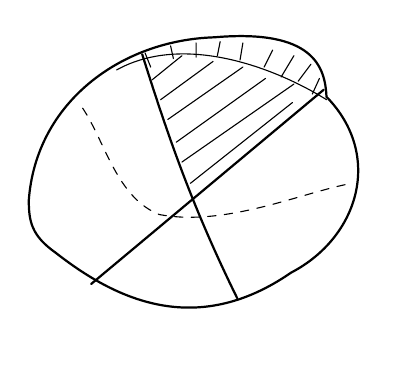
\begin{tikzpicture}[x=0.018cm,y=-0.018cm,line cap=round,line join=round]
\draw[thick] (419,353) .. controls (424,284) and (484,240) .. (550,238) .. controls (620,232) and (628,259) .. (629,280) .. controls (669,321) and (652,379) .. (604,404) .. controls (536,451) and (479,422) .. (438,390) .. controls (421,378) and (419,368) .. (419,353) -- cycle;
\draw[thick] (499,250) .. controls (517,307) and (534,357) .. (566,422) (463,412)--(627,275);
\draw (481,261) .. controls (528,235) and (592,259) .. (629,282);
\draw[dashed] (457,288) .. controls (473,312) and (481,351) .. (511,363) .. controls (558,372) and (613,347) .. (647,341);
\draw (501,249)--(505,259) (519,244)--(521,253) (537,242)--(537,252) (554,241)--(552,251) (570,242)--(568,254) (591,247)--(585,259) (606,251)--(597,266) (618,257)--(609,269) (624,267)--(619,278);
\draw (506,268)--(527,251) (512,282)--(549,255) (517,296)--(570,259) (523,312)--(586,267) (527,326)--(606,271) (533,341)--(605,284);
\end{tikzpicture}}

% crop-candidate: scan 96
\figure{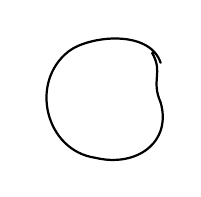
\begin{tikzpicture}[x=0.018cm,y=-0.018cm,line cap=round,line join=round]
\draw[thick] (690,433) .. controls (682,409) and (639,414) .. (625,425) .. controls (597,447) and (609,495) .. (644,500) .. controls (673,507) and (698,489) .. (690,461) .. controls (683,445) and (692,440) .. (684,426);
\end{tikzpicture}}

{\tiny
\begin{verbatim}
****A   END   JOB  338  FATAR                          ROOM        3.01.58 PM 19 AUG 82  R6.PR1    SYS JES2  JOB  338   END   A****
****A   END   JOB  338  FATAR                          ROOM        3.01.58 PM 19 AUG 82  R6.PR1    SYS JES2  JOB  338   END   A****
****A   END   JOB  338  FATAR                          ROOM        3.01.58 PM 19 AUG 82  R6.PR1    SYS JES2  JOB  338   END   A****
****A   END   JOB  338  FATAR                          ROOM        3.01.58 PM 19 AUG 82  R6.PR1    SYS JES2  JOB  338   END   A****
****A   END   JOB  338  FATAR                          ROOM        3.01.58 PM 19 AUG 82  R6.PR1    SYS JES2  JOB  338   END   A****
****A   END   JOB  338  FATAR                          ROOM        3.01.58 PM 19 AUG 82  R6.PR1    SYS JES2  JOB  338   END   A****
\end{verbatim}
}

% crop-candidate: scan 96
\figure{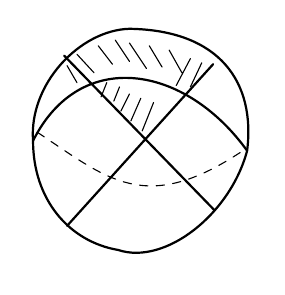
\begin{tikzpicture}[x=0.018cm,y=-0.018cm,line cap=round,line join=round]
\draw[thick] (407,543) .. controls (404,503) and (440,465) .. (475,464) .. controls (539,465) and (564,502) .. (558,550) .. controls (546,595) and (500,631) .. (467,620) .. controls (432,614) and (407,584) .. (407,543) -- cycle;
\draw[thick] (407,543) .. controls (440,477) and (514,489) .. (558,550) (429,483)--(535,592) (431,603)--(534,489);
\draw[dashed] (410,537) .. controls (460,570) and (486,596) .. (555,550);
\draw (431,490)--(438,502) (438,482)--(450,495) (453,476)--(463,489) (465,472)--(475,487) (475,474)--(487,492) (489,476)--(498,491) (503,479)--(512,495) (518,485)--(508,504) (526,488)--(518,505) (459,502)--(455,512) (468,505)--(464,515) (475,510)--(469,522) (483,513)--(476,529) (492,516)--(484,536);
\end{tikzpicture}}

% crop-candidate: scan 96
\figure{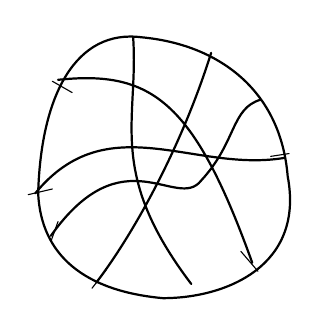
\begin{tikzpicture}[x=0.018cm,y=-0.018cm,line cap=round,line join=round]
\draw[thick] (230,742) .. controls (232,672) and (257,626) .. (303,632) .. controls (357,637) and (401,669) .. (406,730) .. controls (418,793) and (363,816) .. (318,816) .. controls (263,811) and (232,786) .. (230,742) -- cycle;
\draw[thick] (244,662) .. controls (310,655) and (340,677) .. (381,791) (297,632) .. controls (301,691) and (278,727) .. (338,806) (352,643) .. controls (331,710) and (297,771) .. (271,805) (239,772) .. controls (290,700) and (328,755) .. (345,733) .. controls (370,706) and (366,682) .. (387,676) (228,742) .. controls (279,680) and (340,728) .. (404,717);
\draw (240,663)--(254,671) (223,743)--(240,739) (244,762)--(239,776) (268,809)--(278,796) (373,783)--(385,797) (394,716)--(407,714);
\end{tikzpicture}}

% crop-candidate: scan 96
\figure{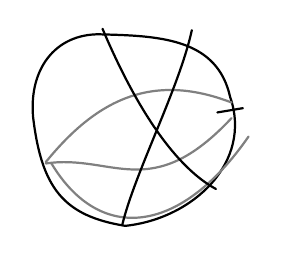
\begin{tikzpicture}[x=0.018cm,y=-0.018cm,line cap=round,line join=round]
\draw[thick] (526,698) .. controls (523,662) and (544,638) .. (576,640) .. controls (618,641) and (656,644) .. (665,684) .. controls (681,730) and (639,770) .. (591,775) .. controls (548,768) and (532,749) .. (526,698) -- cycle;
\draw[gray,thick] (535,730) .. controls (570,687) and (609,666) .. (666,688) (535,731) .. controls (582,724) and (609,760) .. (666,699) (539,731) .. controls (574,789) and (631,780) .. (678,712);
\draw[thick] (575,636) .. controls (603,702) and (631,736) .. (655,749) (638,637) .. controls (629,678) and (598,737) .. (589,774) (656,695)--(674,692);
\end{tikzpicture}}

% crop-candidate: scan 96
\figure{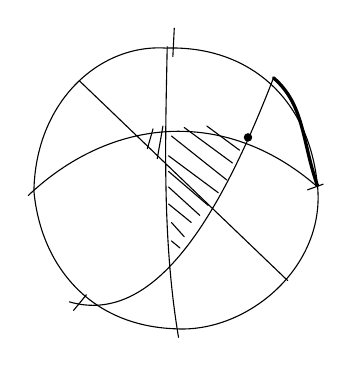
\begin{tikzpicture}[x=0.018cm,y=-0.018cm,line cap=round,line join=round]
\draw[thin] (712,770) .. controls (713,707) and (758,666) .. (805,669) .. controls (862,667) and (906,703) .. (912,766) .. controls (918,823) and (863,870) .. (812,867) .. controls (752,865) and (717,823) .. (712,770) -- cycle;
\draw (744,692)--(891,833) (806,668) .. controls (805,727) and (802,802) .. (814,873) (708,773) .. controls (766,718) and (846,710) .. (911,766) (737,848) .. controls (796,865) and (842,791) .. (881,690);
\draw[very thick] (881,690) .. controls (903,709) and (901,735) .. (912,766);
\fill (863,732) circle[radius=3];\draw (811,655)--(810,675) (740,854)--(749,843) (905,769)--(916,765);
\draw (792,740)--(796,726) (799,747)--(803,724) (809,731)--(848,762) (818,725)--(852,750) (834,724)--(857,741) (807,745)--(842,771) (807,756)--(835,780) (807,767)--(829,787) (807,779)--(823,792) (809,792)--(818,802) (809,805)--(815,810);
\end{tikzpicture}}

% crop-candidate: scan 96
\figure{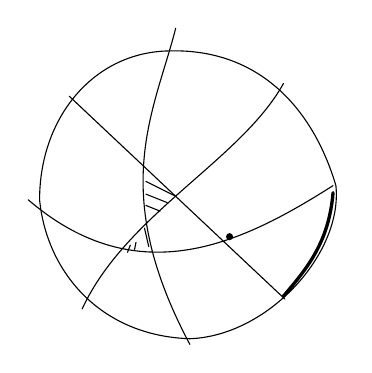
\begin{tikzpicture}[x=0.018cm,y=-0.018cm,line cap=round,line join=round]
\draw[thin] (973,771) .. controls (973,713) and (1011,667) .. (1064,666) .. controls (1128,664) and (1166,707) .. (1182,761) .. controls (1187,809) and (1134,867) .. (1079,869) .. controls (1016,867) and (978,822) .. (973,771) -- cycle;
\draw (994,698)--(1146,841) (1069,650) .. controls (1054,709) and (1021,764) .. (1079,873) (1003,848) .. controls (1034,781) and (1115,743) .. (1145,689) (965,771) .. controls (1043,838) and (1117,801) .. (1180,761);
\draw[very thick] (1180,766) .. controls (1177,801) and (1162,819) .. (1145,839);\fill (1107,797) circle[radius=2.5];\draw (1048,758)--(1068,768) (1048,767)--(1063,773) (1048,775)--(1058,779) (1047,791)--(1050,804) (1041,801)--(1040,806) (1037,803)--(1035,808);
\end{tikzpicture}}

% crop-candidate: scan 96
\figure{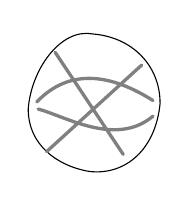
\begin{tikzpicture}[x=0.018cm,y=-0.018cm,line cap=round,line join=round]
\draw (75,845) .. controls (77,817) and (98,788) .. (120,792) .. controls (148,794) and (168,814) .. (168,841) .. controls (165,873) and (144,892) .. (118,889) .. controls (95,885) and (75,870) .. (75,845) -- cycle;
\draw[gray,very thick] (81,840) .. controls (104,816) and (133,820) .. (163,839) (82,845) .. controls (101,850) and (137,872) .. (163,850) (94,805)--(142,877) (88,875)--(155,814);
\end{tikzpicture}}

\scanpage{97}
% archive sheet number: 99

expliciter le lien du paramètre $a$ avec le paramètre $\tau$, ou mieux, avec l'invariant modulaire $j\in\mathbb R^{\unsure{*|?|\pm}}$ (serait-on $j=\unsure{\pm|4|\tfrac12}\log a$ ?) \deleted{i.e. $a=\exp j$ ou $a=\exp -j$, suivant qu'on est dans la famille $E_a$ ou $E'_a$ ?)}.

\figure{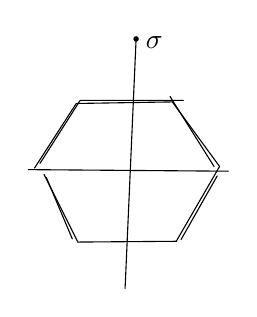
\begin{tikzpicture}[line cap=round]
\draw (0,0)--(.53,.82)--(1.75,.84)--(2.35,.02)--(1.80,-.93)--(.55,-.94)--(.12,-.08);
\draw (.07,.06)--(.58,.86)--(1.89,.86) (1.72,.91)--(2.28,.02) (1.86,-.91)--(2.32,-.10) (.15,-.12)--(.48,-.90);
\draw (-.08,-.02)--(2.46,-.04) (1.15,-1.53)--(1.29,1.64);\fill (1.29,1.64) circle[radius=.035];\node[right] at (1.29,1.59) {$\sigma$};
\end{tikzpicture}}

\deleted{Considérons} Notons que si $\sigma$ est dans $G^-$ alors \inserted{(réflexion par r. à \unsure{un relèvement|une droite} \unsure{orthogonal à celui|orthogonale à celle|hexagonal} de $\sigma$)} suivant les cas $-\sigma$ est conjugué, ou non conjugué, à $\sigma$. Dans le cas hexagonal, il est non conjugué, dans le cas carré, il est conjugué. Dans les cas non extraordinaires, $n=2$, il est bien sûr non conjugué (car $G$ est alors commutatif) --- donc le cas \deleted{hexagonal} \inserted{carré} est le seul où $-\sigma$ \deleted{\unsure{ne|n'}} soit \deleted{\unsure{pas}} conjugué à $\sigma$. \deleted{Donc sauf dans le cas carré peut-être, on trouve}

\uline{Distinguons les cas}

1) \uline{$n=2$} Cas non extraordinaires. Le groupe des autom est $\pm1,\pm\sigma$, où $\sigma$ est un \inserted{anti} autom. On voit de suite que si $\sigma$ est du type somme directe d'un $\mathrm{id}_P$ et $-\mathrm{id}_Q$, il en est de $=$ de $-\sigma$ (avec $P,Q$ échangés) donc on est dans cas $E_a$, ou \deleted{\unsure{$Q$|$a$}} \inserted{${}^a$} dans cas $E_a$ et un $E_{a'}$, correspondant aux deux éléments de $\unsure{\sigma|\sigma,},\sigma'$ de $G^-$, et on aura $aa'=1$. \deleted{\unsure{En|Enf}} en prenant un génér. \inserted{$u=$}$e_+$ de $\unsure{\pi_+|\Gamma_+|\Pi_+}$, un autre, \inserted{$v=e_-$} de $\pi_-$, on a

\[
a=a(\sigma)=\frac{Q(e_-)}{Q(e_+)}
\]

et comme par passage de $\sigma$ à $-\sigma$ \deleted{les} $e_+$ et $e_-$ s'interchangent, on aura bien

\margin{Ceci vaut aussi bien dans les cas des $E_a$, que des $E'_a$}

\[
a(-\sigma)=1/a(\sigma)
\]

(valable dans tous les cas), donc

\[
a(-\sigma)=a(\sigma)\Longleftrightarrow a(\sigma)=1\Longleftrightarrow\text{Cas \uline{carré}}.
\]

\scanpage{98}
% archive sheet number: 100

2) \uline{Cas carré} $n=4$. On voit que l'on a une $\sigma$ du type $E_1$, et $-\sigma$ est du $=$ type. La $\unsure{2^{\mathrm e}|2}$ correspond aux symétries p. r. aux \deleted{\unsure{segments|sommets}} \inserted{diagonales} du carré du départ. La symétrie par rapport à une \unsure{arête|côté} échange $e_0$ et $e_1$, les invariants et anti-invariants sont resp. engendrés par $e_0+e_1$ et $e_0-e_1$, qui n'engendrent \uline{pas} le \deleted{\unsure{ré|rése}}réseau, donc on est dans le cas $E'_{\unsure{a|1|a'}}$. On a

\figure{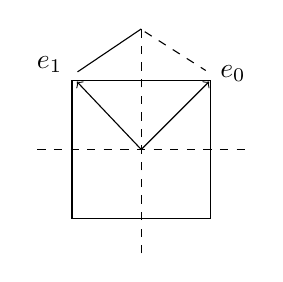
\begin{tikzpicture}[x=.88cm,y=.88cm]
\draw (-1,-1)--(1,-1)--(1,1)--(-1,1)--cycle;
\draw[dashed] (-1.5,0)--(1.6,0) (0,-1.5)--(0,1.75);
\draw[->] (0,0)--(-.93,.98);\draw[->] (0,0)--(.98,.98);
\draw (-.92,1.12)--(0,1.74);\draw[dashed] (.05,1.70)--(.93,1.14);
\node[left] at (-1,1.23) {$e_1$};\node[right] at (1,1.10) {$e_0$};
\end{tikzpicture}}

\margin{\deleted{\unsure{$E$|$E'$}} \unsure{les|cas}}

\[
a'=\frac{Q(e_0-e_1)}{Q(e_0+e_1)}=\deleted{\unsure{4|1|A}}1\quad\text{aussi}
\]

Donc on trouve les types $E_1$ (``sommets'') et $E'_1$ (``côtés'',

3) \uline{Cas hexagonal} $n=6$. \deleted{\unsure{Sy|S}} \uline{Réflexions-sommets}. Les \deleted{\unsure{som|inv}} invariants pour la réflexion p. r. à $\mathbb R u$ sont engendrés par $u$, les anti-invariants par $2v-u$, c'est du type $E'_a$, avec

\figure{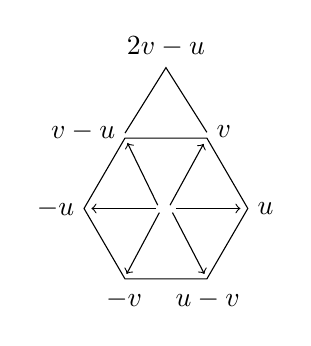
\begin{tikzpicture}[x=1.04cm,y=1.04cm]
\draw (-1,0)--(-.50,.86)--(.50,.86)--(1,0)--(.50,-.86)--(-.50,-.86)--cycle;
\draw (-.50,.92)--(0,1.72)--(.5,.93);
\draw[->] (-.10,.04)--(-.47,.80);\draw[->] (.05,.04)--(.46,.79);\draw[->] (-.12,0)--(-.91,0);\draw[->] (.12,0)--(.91,0);\draw[->] (-.08,-.05)--(-.48,-.80);\draw[->] (.08,-.05)--(.47,-.80);
\node[above] at (0,1.73) {$2v-u$};\node[left] at (-.5,.94) {$v-u$};\node[right] at (.5,.94) {$v$};\node[left] at (-1,0) {$-u$};\node[right] at (1,0) {$u$};\node[below] at (-.51,-.88) {$-v$};\node[below] at (.51,-.88) {$u-v$};
\end{tikzpicture}}

\[
a=\frac{Q(2v-u)}{Q(u)}=\sqrt{3}
\]

\uline{Réflexions-faces} Ce sont les $-\sigma$, on trouve donc $E'_{1/a}=E'_{1/\sqrt{3}}$.

\uline{En résumé}. Dans tous les cas, sauf le cas carré, \deleted{toutes} \inserted{l'une des} \deleted{les} \inserted{les types de} structures réelles sur $X$ sont soit \deleted{du type} $\{E_a,E_{1/a}\}$, \deleted{t cas} soit $\{E'_a,E'_{1/a}\}$ \inserted{avec $a>1$} (le cas hexagonal étant dans le deuxième cas \inserted{avec $a=\sqrt{3}$}), à l'exclusion bien sûr l'une de l'autre. \uline{Dans} le cas carré, l'ens des structures réelles est $\{E_1,E'_1\}$ i.e. il y a à la fois des structures $E$ et $E'$.

\scanpage{99}
% archive sheet number: 101

\uline{Résumé}\quad Cas $E_a$ :

\[
\left|\begin{aligned}
&\text{base}\quad u=e_0,\ v=e_1\\
&\text{forme}\quad\deleted{Q(e_0)=Q(e_1)}\quad Q(xe_0+ye_1)=x^2+ay^2
\end{aligned}\right.
\]

Si on veut \deleted{\unsure{l'on|la}} faire $Q$ sous forme ``\unsure{standart|standard}'', on prend la \inserted{nouvelle} base $\underbrace{e_0}_{1},\underbrace{\frac{1}{\sqrt a}e_1}_{i}$, on trouve donc la base $1,\sqrt a\,i$ d'où

\[
\boxed{\tau=\sqrt a\,i}.
\]

Cas $E'_a$ : base $u,v$, \deleted{\unsure{$e_0,e_1$ étant les|les $e$ étant les|$e_0$, $v=$}} \inserted{\unsure{forme|formes}} distingués p. r. à la base

\[
\begin{aligned}
&e_0=u,\ e_1=2v-u\,;\qquad Q(xe_0+ye_1)=x^2+ay^2\\
&v=\tfrac12(e_0+e_1):
\end{aligned}
\]

on \deleted{\unsure{passe encore|passe encore une}} change encore de base $\underbrace{e_0}_{1},\underbrace{\frac{1}{\sqrt a}e_1}_{\unsure{i|v}}$ base orthonormale et on a $u\Rightarrow1,\ v\longmapsto\frac12(1+\sqrt a\,i)$, donc

\[
\boxed{\tau=\frac12(1+\sqrt a\,i)}=\frac12+\frac{\sqrt a}{2}i
\]

\figure{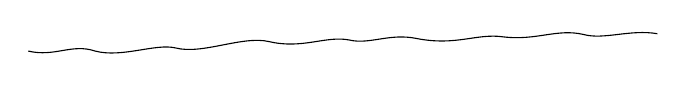
\begin{tikzpicture}[x=.85cm,y=1cm]\draw (0,0) .. controls (.4,-.08) and (.65,.10) .. (1,0) .. controls (1.4,-.09) and (1.9,.1) .. (2.2,.04) .. controls (2.6,-.05) and (3.2,.20) .. (3.6,.12) .. controls (4.1,.02) and (4.45,.20) .. (4.8,.14) .. controls (5.1,.08) and (5.4,.23) .. (5.8,.16) .. controls (6.4,.06) and (6.7,.23) .. (7.1,.18) .. controls (7.6,.13) and (7.9,.29) .. (8.3,.21) .. controls (8.6,.14) and (9,.28) .. (9.4,.22);\end{tikzpicture}}

Calcul \unsure{du groupe|des groupes} des pts réels d'une courbe $E_a,E'_a$.

Pts réels sont les : $x\bmod\pi$ ($x\in\pi_{\mathbb R}$) tels que

\[
\sigma x\equiv x\quad(\pi)
\]

\uline{Distinguons les deux cas}. 1) \uline{$E_a$}\quad $\deleted{\sigma(e_0,e_1)=}\ \sigma(x,y)=x,-y$

\[
\text{donc}\qquad \sigma(x,y)-(x,y)=(0,2y)
\]

donc la condition est que $2y\in\mathbb Z$. Donc il y a \deleted{\unsure{outre|out|ou}} les pts de \deleted{$\unsure{0,\frac12|0,\frac12e|0,}$} $\mathbb R e_0$ et de \deleted{$\unsure{\mathbb R|R_1}$} $(\unsure{0|b},\tfrac12)+\mathbb R e_0$, donc \uline{deux composantes} \uline{connexes} \uline{pour} $X(\mathbb R)$.

\scanpage{100}
% archive sheet number: 102

\uline{Cor} Supposons $k$ principal, \inserted{$2$-régulier} $k_0=k/2k$ un corps. Alors les \inserted{\unsure{cl. d'isom|cl. de tels|à isom. près}} $(M,\sigma)$ précédents reviennent à : celles des paires $(P,Q,\deleted{\unsure{p,q,m|p,q}})$ avec $P,Q$ libres de rang $1$, et \deleted{\unsure{$p\,q$|$p$|$p\subset$}} $m\subset\underbrace{P/\unsure{2|k}P}_{p}\oplus\underbrace{Q/2Q}_{q}$ sous-esp. vectoriel sur $k_0$, \deleted{\unsure{de tel que|du tel que}} qui est soit nul, soit une droite $\ne p,q$ (droites coordonnées)

\uline{Cor} Cela donne une classification des classes de conjugaison d'éléments de $\mathrm{Gl}(2,k)\deleted{\unsure{^*|^-}}$ qui sont d'ordre $2$ exactement, et distincts de $\{\pm1\}$ : il y \deleted{en a} a \inserted{celle de} $\left(\begin{smallmatrix}1&0\\0&-1\end{smallmatrix}\right)$ (correspondant au cas $m=0$), puis \uline{une} \deleted{\unsure{famille entière|famille indexée|familles indexées} par l'ens des \unsure{points|gens} de $\mathbf P^1(k_0)$ distincts de $0,\infty$ (en supposant que $k^*\to k_0^*$ est surjectif, sinon la classification sera plus fine,} \inserted{en supposant que $k^*\to k_0^*$ surj, on} peut via des bases de $P/2P$ resp. $Q/2Q$ se ramenant à une base de $P,Q$.

Elle correspond à

\[
\begin{aligned}
&P=k,\ Q=k,\ m=\text{diagonale de }k_0\times k_0\quad\text{i.e.}\\
&M'=(2k\oplus2k)+\operatorname{diag.}\text{ de }k\oplus k=\{(x,y)\mid x-y\in2k\}
\end{aligned}
\]

donc on peut prendre base de $M'$

\[
\unsure{u|e_u|u_0}=(2,0),\quad\unsure{v|e_v|v_1}=(1,1),\quad\text{d'où}\quad -u+2v=(0,2)=\text{sym}(u)
\]

\margin{$u=2e_0$\\ $v=e_0+e_1$}

On trouve

\[
\sigma u=u,\quad \sigma v\ \deleted{\unsure{\ne|+|=}}(1,-1)=u-\mathrm{sym}\,v=u-v
\]

i.e. la matrice de $\sigma$ p. r. à $(u,v)$ est

\[
\begin{pmatrix}1&1\\0&-1\end{pmatrix}
\]

Dans le cas de $k=\mathbb Z$, c'est la matrice de la réflexion p. r. à la diagonale $0,e_0$ de l'hexagone régulier, la fig. de l'hexagone étant rapporté à un syst. de coordonnées obliques ayant comme base deux sommets consécutifs $u,v$ ($M$ est le réseau engendré par l'un des sommets).

\figure{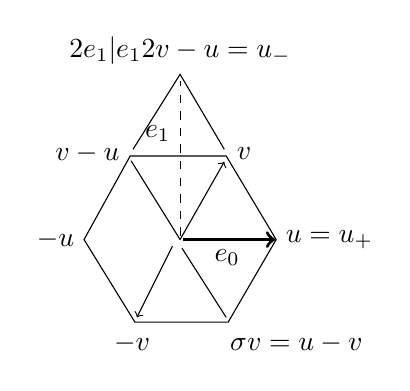
\begin{tikzpicture}[x=1.22cm,y=1.22cm]
\draw (-1,0)--(-.52,.87)--(.48,.87)--(1,0)--(.50,-.86)--(-.47,-.86)--cycle;
\draw (-.49,.94)--(0,1.72)--(.46,.94);
\draw[->] (0,0)--(.46,.81);\draw[->,very thick] (.03,0)--(.99,0);\draw[->] (-.08,-.07)--(-.45,-.81);\draw (0,0)--(-.51,.82) (.02,-.09)--(.48,-.81);
\draw[dashed] (0,.04)--(0,1.65);
\node[above] at (0,1.72) {$\deleted{\unsure{2e_1|e_1}}2v-u=u_-$};\node[left] at (-.53,.9) {$v-u$};\node[right] at (.49,.90) {$v$};\node[left] at (-1,0) {$-u$};\node[left] at (0,1.1) {$e_1$};\node[below] at (.49,0) {$e_0$};\node[right] at (1,0) {$u=u_+$};\node[below] at (-.50,-.88) {$-v$};\node[below right] at (.42,-.89) {$\sigma v=u-v$};
\end{tikzpicture}}

\margin{\uline{NB} Soit $u_+$ une base de $\pi_+$, $u_-$ une base de $\pi_-$, alors \deleted{dans} On peut représenter $\sigma_{\mathbb R}$, pour la base $(u_+,u_-)$ de $\pi\otimes_{\mathbb Z}\mathbb R$ par la matrice $\left(\begin{smallmatrix}1&0\\0&-1\end{smallmatrix}\right)$ le réseau $\pi$ étant identifié à $\mathbb Zu_-+\mathbb Zu_+$ \inserted{$\simeq\mathbb Z^2$} dans le premier cas, et dans le $2^{\text{ème}}$ à l'ens des $\unsure{x|a}u_++yu_-$ tels que $x-y\in\mathbb Z$, $x,y\in\frac12\mathbb Z$}

\margin{$\sigma^2(e_1)=\sigma e_0-\sigma e_1=e_0-(e_0-e_1)=e_1$}

\scanpage{101}
% archive sheet number: 103

2) \uline{$E'_a$} Donc $\pi$ engendré par $u,v$ avec $\sigma u=u,\ \sigma v=u-v$

\[
\begin{aligned}
&\sigma(x,y)=\sigma(xu+yv)=xu+y(u-v)=(x+y)u-yv.\\
&\sigma(x,y)-(x,y)\unsure{\equiv|=}yu-2yv=y(u-2v),
\end{aligned}
\]

donc la condition est $y\in\mathbb Z$ ; donc on trouve \deleted{que} les points de $\mathbb R\unsure{u|e_0|u_+}$ mod $\pi$, donc dans ce cas $X(\mathbb R)$ est connexe.

\margin{$9.2$}

\uline{NB} Pour bien faire, il faudrait aussi classifier les courbes elliptiques réelles inhomogènes, i.e. les torseurs (sur $\operatorname{Spec}\mathbb R$) sous les \inserted{schémas en} groupes elliptiques $E_a,E'_a$. Les torseurs non triviaux fournissent les surfaces conformes \deleted{sans} bord non orientables de genre $1$. La suite exacte de $\sigma$-modules (où $\gamma=\operatorname{Gal}(\mathbb C/\mathbb R)\simeq\{\pm1\}$)

\diagram{\begin{tikzcd}[ampersand replacement=\&,column sep=small]
0\arrow[r,dash]\&\pi\arrow[r,dash]\&V\arrow[r,dash]\&E(\unsure{\mathbb C|\deleted{\mathbb C}})\arrow[r,dash]\&0
\end{tikzcd}}

fournit

\[
H^1(\gamma,E(\mathbb C))\simeq H^2(\gamma,\pi)\simeq\pi^\gamma/(1+\sigma)\pi=\pi_+/(1+\sigma)\pi
\]

1) Cas de $E_a$. On a $\pi\simeq\pi_+\oplus\pi_-$, d'où $\pi^\gamma=\pi_+$

\[
H^1(\mathbb R,E_{\mathbb R})\simeq H^1(\gamma,E(\mathbb C))\simeq H^2(\gamma,\pi)\simeq
\underset{\Vert\,\mathbb Z/2\mathbb Z}{\underline{H^2(\gamma,\pi_+)}}\oplus
\underset{\Vert\,0}{\underline{H^2(\gamma,\pi_-)}}
\]

Il y a exactement un élément non nul dans $H^1$, qui est d'ordre $2$

2) Cas de $E'_a$. On a $H^1(\mathbb R,E_{\mathbb R})\simeq0$.

Donc les seules courbes elliptiques vraiment inhomogènes sur $\mathbb R$ sont les $E_a^{!}=$ \inserted{les} torseurs \deleted{\unsure{tr|ts}} non triviaux (d'ordre $2$) sous $E_a$, dépendant du paramètre $a\in\mathbb R^{*+}$.
